% ==========================================
% SECTION 8.9: INTERPRETING THE TRANSFORMER
% ==========================================
\section{8.9. Interpreting the Transformer}

\begin{frame}{Nội dung trình bày}
	\tableofcontents[currentsection]
\end{frame}

% SLIDE: 8.9.1 In-context learning
\begin{frame}{8.9.1. In-Context Learning and Induction Heads}
Ta có một số định nghĩa sau:
		\begin{itemize}
			\item \textbf{Pretraining}: mô hình cập nhật tham số bằng gradient descent để giảm loss.
			\item \textbf{Prompting}: không thay đổi trọng số, mô hình chỉ tận dụng thông tin có sẵn trong context khi suy luận.
			\item \textbf{In-Context Learning} có thể hiểu là khả năng mô hình học cách làm task mới ngay trong inference, mà không cần bất kỳ bước cập nhật tham số nào.
		\end{itemize}
\end{frame}

\begin{frame}{8.9.1. In-Context Learning and Induction Heads}
	Vậy \textbf{In-Context Learning} hoạt động như nào?
	
	$\rightarrow$ Cơ chế chính xác của in-context learning \textbf{vẫn chưa được hiểu hoàn toàn}, nhưng một giả thuyết nổi bật là vai trò của \textbf{induction heads}.
	
	\vspace{0.5cm}
	
	\pause
	\textbf{Chức năng chính} của induction heads là hỗ trợ \textbf{dự đoán các pattern} lặp trong chuỗi:
	\begin{itemize}
		\item Khi gặp một token ở hiện tại, mô hình tìm về lần xuất hiện trước đó của token này.
		\item Sau đó nó có xu hướng “copy” token từng đi sau nó ở quá khứ để dự đoán token tiếp theo.
	\end{itemize}
	
	\vspace{0.5cm}
	\pause
	Các nghiên cứu \textbf{ablation} cho thấy khi làm yếu hoặc loại bỏ induction heads, khả năng in-context learning giảm rõ rệt. Điều này cho thấy chúng có \textbf{liên quan quan trọng}, dù chưa giải thích toàn bộ hiện tượng.
\end{frame}

\begin{frame}{8.9.1. In-Context Learning and Induction Heads}
	\begin{figure}
		\centering
		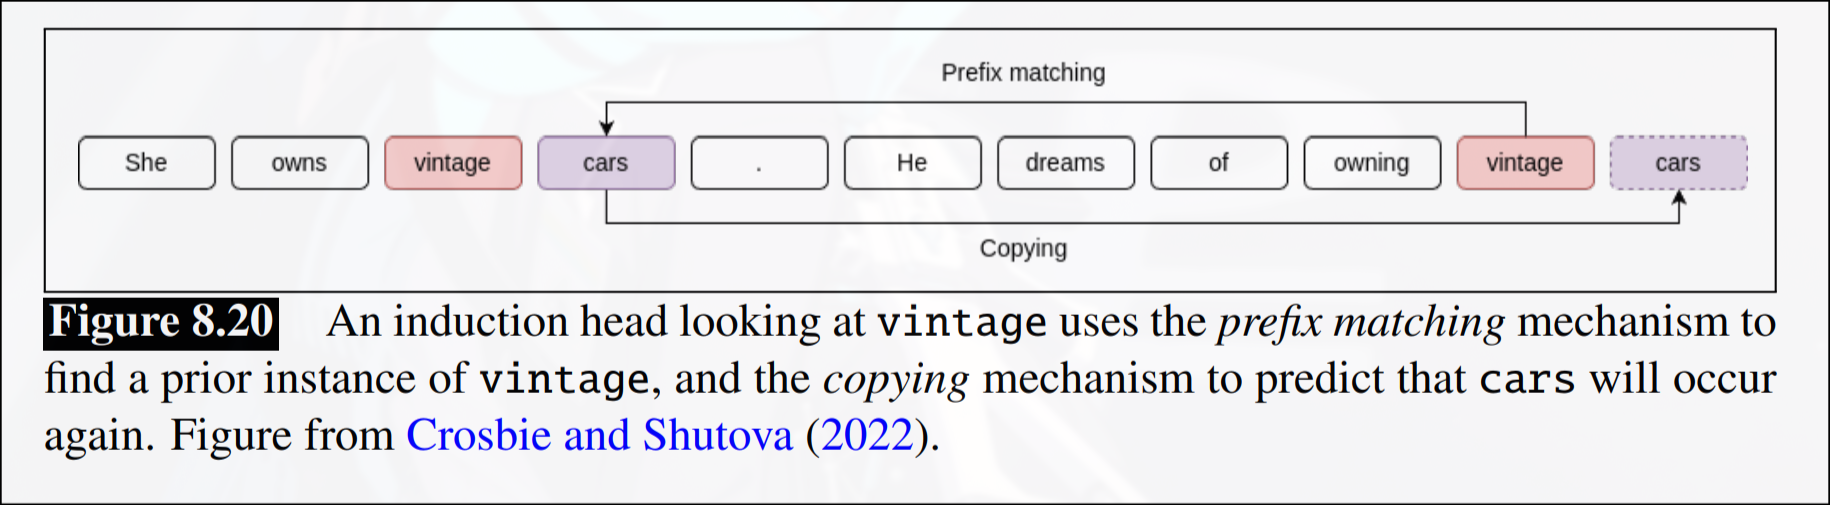
\includegraphics[width=1\linewidth]{img/figure8_20}
	\end{figure}
\end{frame}

% SLIDE: 8.9.2 Logit Lens
\begin{frame}{8.9.2. Logit Lens}

		\textbf{Mục tiêu:} Quan sát quá trình hình thành dự đoán \textbf{bên trong các lớp ẩn}, thay vì chỉ nhìn output cuối cùng.
		\vspace{0.3cm}
		\begin{itemize}
			\item Lấy \textbf{vector trạng thái ẩn} tại một lớp trung gian bất kỳ.
			\item Chiếu trực tiếp vector này lên \textbf{không gian từ vựng} bằng ma trận giải nhúng $E^T$.
			\item Giúp visualize mô hình đang "nghiêng"\ về từ nào ở từng giai đoạn xử lý.
		\end{itemize}


\end{frame}


\section{8.10. Summary}

\begin{frame}{Nội dung trình bày}
	\tableofcontents[currentsection]
\end{frame}

\begin{frame}{8.10. Summary}

\begin{itemize}
	\item Transformer là kiến trúc không hồi quy, dựa trên multi-head self-attention để mô hình hóa quan hệ giữa các token trong ngữ cảnh.
	\vspace{0.5cm}
	\item Một transformer block gồm residual connection, layer normalization, multi-head attention và feed-forward; nhiều block được xếp chồng để tăng năng lực biểu diễn.
	\vspace{0.5cm}
	\item Đầu vào của transformer là tổng của token embedding và positional encoding để mô hình biết cả nội dung lẫn vị trí của token.
	\vspace{0.5cm}
	\item Trong language model, đầu ra từ tầng cuối được chiếu qua unembedding matrix để tạo logits, rồi qua softmax để dự đoán xác suất token tiếp theo.
	\vspace{0.5cm}
	\item Transformer-based language models có thể xử lý ngữ cảnh rất dài, nhờ đó tận dụng được nhiều thông tin hơn khi dự đoán.
\end{itemize}
\end{frame}
